\documentclass[12pt]{article}

%\oddsidemargin=.05in
%\evensidemargin=.05in
%\topmargin=-0.0in
%\textwidth=6.5in
%\textheight=8in
%\pagestyle{empty}

\usepackage{multicol}
\usepackage{amsmath,amssymb,amsthm}
\usepackage{easylist}
\usepackage{graphicx}
\newtheorem*{theorem}{Theorem}
\newtheorem*{claim}{Claim}
\newtheorem*{proposition}{Proposition}
\renewcommand{\qedsymbol}{\ensuremath{\blacksquare}}
\usepackage{fancyhdr}
\pagestyle{fancy}
\fancyhf{}
\lhead{Math 480 Project}
%\chead{Captain Scheduling for Ride the Ducks}
\rhead{Bickel and Yoon}
\cfoot{\thepage}

\usepackage{titlesec}

\titleformat{\section}
  {\normalfont\fontsize{15}{15}\bfseries}{\thesection}{1em}{}
\titleformat{\subsection}
  {\normalfont\fontsize{12}{15}\bfseries}{\thesection}{1em}{}

\begin{document}

\title{Captain Scheduling for Ride the Ducks of Seattle} 

\author{Zach Bickel and Michael Yoon}
\date{March 18, 2015}
\maketitle

\begin{abstract}
This paper describes the model and solution we derived from a scheduling problem for a 
small business, Ride the Ducks of Seattle. Our task was to create scheduling 
software that satisfied the needs of the 
company as well as the workers. The problem is modeled as a Mixed Integer Program. After simplifying the problem at hand, we were able to derive decision variables and constraints. We modified an existing algorithm to fit our needs in finding a feasible solution to our scheduling problem. Our finished product will be used 
by Ride the Ducks and will be flexible enough to fit their week-to-week 
schedule making process.
\end{abstract}


%\begin{multicols}{2}
\section*{Background}
Ride the Ducks of Seattle offers continuous tours of downtown Seattle every day of the year except for Christmas, Christmas Eve and Thanksgiving. The Land \& Water Tour is a 90-minute tour that begins from two separate locations in downtown Seattle. Each tour is directed by a Captain, who operates an amphibious vehicle called a DUKW, colloquially known as a duck, used during World War 2. After each 90-minute tour is finished, there is a 30-minute break period for de-boarding the current tour before boarding the next tour, all while providing a small break for the Captain. Each Captain will usually work 5 tours a day, 4 days a week, although there is a lot of deviation from this in practice. Throughout this paper, we refer to 2-hour tour blocks, or simply 2-hour blocks, to denote a 90-minute tour followed by a 30-minute break period.


Scheduling problems are very common for small businesses where many managers are still doing it by hand. Ride the Ducks of Seattle usually opens at 9:00 AM and closes at 9:00 PM, running tours from 9:20 AM to 7:20 PM, meaning that their scheduling problems are fairly large. Management at Ride the Ducks of Seattle currently spends upwards of ten hours per week scheduling captains for tours. Our task is to build scheduling software that will drastically cut this time down and automatically build a schedule. This will be flexible enough so that a user will be able to update the constraints as they change. 


\begin{figure}[h!]
\centering
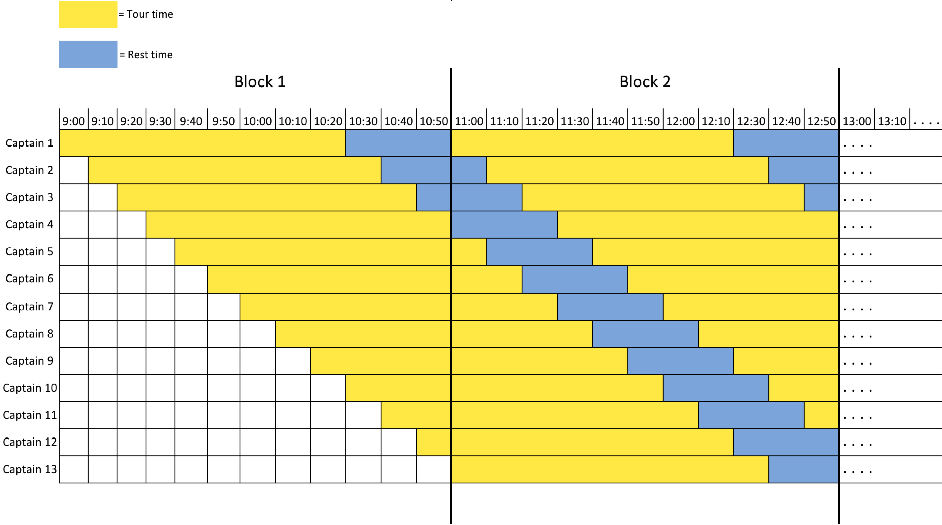
\includegraphics[scale=0.7]{block_figure2.png}
\caption{Staggered Block Structure}

\end{figure}

Scheduling the Captains in a way that satisfies the company as well as the 
individual Captains can be tricky. There are individual captain constraints that we have to deal with while filling the tours Ride the Ducks wants to run. Captain constraints can vary week to week and the amount of tours run in a day depends seasonally with the warmer seasons needing more tours than the cooler seasons. Due to the need of a flexible scheduling system, making the scheduling software easy to edit is crucial. The company can then 
make their own schedules with changing constraints and objectives.

\section*{Goal}
Our goal is to automate a scheduling system for the Captains of Ride the Ducks to cover all tours while satisfying each Captain's individual constraints. Note that we are simply attempting to find a feasible solution rather than an optimal one since we do not have a clear objective function. % and attempting to minimize 4-day stretches.

\section*{Simplifications}
We started with an example Ride the Ducks schedule. The schedule is broken down into which captains are working what days and the times that day a Captain will be running a tour. The schedule also gives one or two captains that are on-call. From the schedule given by the company, we were able to break down the schedule into the decisions Ride the Ducks has to make when building a schedule. The decisions include how many captains we want working in a day, how many tours we want to run at a specified time, all while paying attention to individual Captains restrictions. 

There are two different locations where tours take off, however we have not differentiated them in our model. The two different locations run the same tour, so modeling as one location is sufficient. We also chose to extend possible tour times from 9 AM to 9 PM for future flexibility. With this extension to the model, we were able to simplify the blocks of tours to six 2-hour blocks of tours per day. 

We made further assumptions to certain aspects of the variables involved. For the tours, we assumed that they run on time and would not run over the 2-hour allotment. The available time slots in the model are set to a default of every 10 minutes. So, tours can be run every 10 minutes, if needed. This allows for the most time slots per 2-hour block these captains are working in.  
Rather than count the number of hours a Captain works per week, we only keep track of the number of days a captain has worked. Due to our block structure, we are able to implicitly keep track of the number of hours they work. The number of 2-hour blocks in a day is maxed out at 6. For the most part, captains will work 4 days, touring in 5 blocks each day, coming to 40 hours per week.

Currently, the model does not include on-call workers, it simply creates a schedule where all captains are assigned days where they are touring. Since on-call days are not counted as worked days when the schedule is initially made and there are separate constraints involved, assigning captains to this role has been left open by our model. These simplifications allow us to create our decision variables and constraints in a clear way so we can tackle our problem.

\section*{Literature Overview}
Before we tried to model the problem at hand, we read research papers on modeling problems similar to our own. One paper we came across discussed a model built by a team from America West Airlines and Arizona State University used to decide on an optimal airplane boarding strategy (Van Den Briel, 2002). We gained insight on handling Mixed Integer Problems from reading about how the modeling team tackled the problem. This helped us better identify the decision variables and constraints in our own problem. It also helped us to understand how to simplify our own constraints. Simplifying the problem gave us more flexibility on how to represent Captains and time slots.

We too wanted to model our scheduling problem using Integer Programming. A relevant paper by Nicholas Beaumont on scheduling problems using Integer Programming served as inspiration (Beaumont, 1997). In Beaumont's case study, the staff he was trying to schedule had many similarities to the staff we were trying to schedule. This included constraints on the staff based on times they could work and the demand of their work (Beaumont, 1997). Using binary values and other variables assigned to certain staff members to restrict their start times was something that we wanted to implement in our model. These constraints change weekly for our own partner, thus fully understanding the formulation of these constraints was necessary to construct code that would create these constraints for our partner once we hand them our final product. These papers offered us guidance on our own problem and model and helped us formulate it as an Integer Program.

A paper done on scheduling for the Math Study Center at the University of Washington was another similar modeling problem (White, 2004). Their solution generated optimal weekly timetables for tutors at the Math Study Center using similar constraints to our problem. The modeling team chose to formulate the scheduling problem as an Integer Program that used a two-step process. The first step of their modeling process involved finding a feasible solution that satisfied all constraints. If no feasible solution was found in the first step, they used an iterative approach to relax individual constraints until one was found. Once a feasible solution was found, they used a second step to improve on the schedules. The team implemented a branch and bound algorithm in order to optimize an objective function. This step improves upon the initial schedule with employee preferences in mind. We took this two-step process and modified it to better fit our model where we have no objective function and are simply finding a feasible solution. 

\section*{Variables and Parameters} First, let's define some parameters:
\begin{align*}
n &\equiv \text{Number of captains,}\\
m &\equiv \text{Number of tour slots per 2-hour block,}\\
b &\equiv \text{Number of 2-hour blocks in one day,}\\
k &\equiv \text{Number of time slots per day.}
\end{align*}
If there are $n$ captains and $k$ time slots in a day, then there are $7kn$ decision variables. Note that $k = mb$. Our decision variables will represent when the captains will run a tour. We can understand them as a matrix $X$, where $x_{ijd}$ = 1 if captain $i \in \{1, 2, \dots, n\}$ runs a tour at time $j \in \{1, 2, \dots k\}$ on day $d \in \{1, 2, \dots, 7\}$, and 0 otherwise.

%\section*{Objective Function}
%Our objective function will represent the number of 4-day stretches captains have to work and our goal will be to minimize this %in order to keep captain fatigue low. For readability purposes, let's define a separate function $w(i, d)$ to represent captain %$i$ working on day $d$:
%$$w(i,d) = \sum_{j = 1}^{k}{x_{ijd}}.$$
%So, $w(i,d) = 1$ if captain $i$ works on day $d$ and 0 otherwise. Then $w(i, 1)w(i, 2)w(i, 3)w(i, 4) = 1$ implies that captain %works on days 1, 2, 3 and 4. Our objective function $f$ is thus:
%$$f(i) = [w(i, 1) \cdots w(i, 4)] + [w(i, 2) \cdots w(i, 5)] + \cdots + [w(i, 4) \cdots w(i, 7)] + [w(i, 5) w(i, 6) w(i, 7) %w(i,1)].$$
%Note that the last term in the function wraps around to make sure that we are not loading the schedule too heavily towards the %weekend shifts.

\section*{Constraints}
For simplification, assign
$w_{id}$ to be 1 if Captain $i$ works on day $d$ and 0 otherwise. So, for Captain $i$ on day $d$, 

$$w_{id} = \begin{cases} 1 & \mbox{if } \sum_{j = 1}^{k}x_{ijd} \ge 1,\\
0 & \mbox{otherwise}. \end{cases}$$

\begin{enumerate}
\item[(1)] Captain requested tours constraint: Ride the Ducks offers special tours for large groups (birthdays, corporate events,  etc.). Some captains are requested by name to run these specific tours. So if captain $i$ is requested on
day $d$ at time slot $j$,
$$x_{ijd} = 1.$$
\item[(2)] Time between tours constraint: A Captain needs 2-hours between each of their tours in a given day. 
If Captain $i$ runs tours at time slots $j$ and $j'$ on day $d$, such that $j \neq j'$,
$$\lvert j - j'\rvert \ge m.$$
Ideally, this would be an equality constraint, but constraint (6) may make this impossible if a Captain is requested to run several tours that are on different cycles of the 2-hour block structure (i.e. runs 9:20 and 12:00 rather than 9:20 and 11:20). 
\item[(3)] Number of days worked per week constraint: For the most part, each captain can work a maximum of 4 days per week although it can vary. We'll define the maximum number of days captain $i$ can work as $y_i$.
For each captain $i$,
$$\sum_{d = 1}^{7}w_{id}\le y_i.$$
\item[(4)] Captain unavailability constraint: If captain $i$ is unavailable on day $d$,
$$\sum_{j = 1}^{k}{x_{ijd}} = 0.$$
\item[(5)] Tours per day for each Captain constraint: A Captain works 5 tours per day. So, for Captain $i$ on day $d$, 
$$\sum_{j = 1}^{k} x_{ijd} = 5.$$
\item[(6)] Tours per time slot constraint: We would like to have a certain number of tours starting at each time slot. If we want $t_{jd}$ tours at time slot $j$ on day $d$,
$$\sum_{i = 1}^{n}{x_{ijd}} = t_{jd}.$$
\item[(7)] Number of daily captains constraint: We want to have $c_d$ captains at work on day $d$. This means that, for day $d$, 
$$\sum_{i = 1}^{n}{w_{id}} = c_d.$$
\end{enumerate}
Constraints (1) through (5) are individual Captain constraints while constraints (6) and (7) are company constraints. Note that we do not have constraints for hours worked per day or week since they are implied by (1)-(5), especially by (3) and (5).

\section*{Algorithm and Commentary}
The algorithm we used to obtain a feasible solution is similar to the one used in White, 2004. It involves assigning tours in the fashion of a greedy algorithm, paying attention to Captain constraints (1)-(5), with the goal fulfilling constraints (6) and (7). Since we utilize a greedy algorithm, constraints (6) and (7) may not be met with one pass, so we implemented an approach that would use multiple passes and relax constraints as needed to get a feasible solution. Steps to the algorithm are set in italics and commentary is set in normal font. 

\begin{itemize}
\item[(1)] \textit{If a Captain has requested tours, assign them their requested tours, satisfying constraint (1). For each day where a Captain has requested tours, fill in the Captain's schedule for that day, so that they work a full five tours, while work towards fulfilling constraint (6).}

Note that the requested tours may occur off-cycle. For example, a Captain has requested tours at 9:20 in the morning and 12:00 in the afternoon. In this case, the Captain will need a longer break in order to get onto a new cycle (i.e. runs 9:20 and 12:00 rather than 9:20 and 11:20). 

\item[(2)] \textit{Loop through every Captain on each day for each tour time slot. If the Captain is not scheduled the day before or after, no individual constraints are violated, and a tour is unfilled at that particular time slot on that day, then assign the Captain to the particular tour.}

Note that this fills Captains into tours so that they don't have to work two days in a row in a given week. This step essentially breaks the captains into two groups and has each group run on alternate days. Because of the nature of the captain constraints, we will not be able to fully break the captains into alternating groups and fully satisfy constraints (6) and (7), so we'll have to go through the captains again without the alternating scheme to fill in more tours.

\item[(3)] \textit{Loop through every Captain on each day for each tour time slot. If no individual constraints are violated and a tour is unfilled at that particular time slot on that day, assign the Captain to the particular tour.}

In this step, we are filling in what the alternating scheme could not fill in from part (2). This attempts to fill in all open tours with Captains whose individual constraints would not be violated by assigning them to unfilled tours. If a feasible schedule exists, it will be found in this step.

\item[(4)] \textit{If there are still unfilled tours, relax individual constraints  (first (3), then (4)) and give a report to management so they can make an informed decision about covering unfilled tours.}

In this step, we are filling in what the alternating scheme could not fill in from part (3).
\end{itemize}


\section*{Results} 

\begin{figure}[h!]
\centering
\includegraphics[scale=0.9]{"Example_Schedule".png}
\caption{Example of Captain Schedule.}
\end{figure}
\noindent The schedules being created by our code are feasible. They stay within the constraints for all schedules as well as complying with individual constraints set by captains themselves. Our first schedules were more automated and did not include any of the individual captains constraints. The schedules satisfied the number of tours and captains per day, tours per time slot, and number of days worked. The captains were being assigned in two groups that alternated. This allowed for a feasible schedule based on most of Ride the Ducks' constraints. This also allowed for captains to be rested between days they worked. Of course, these schedules are not entirely feasible since they do not satisfy all of the individual constraints. We then added the individual constraints and we see the schedule created by our code.  This schedule satisfies more of the individual constraints while satisfying most of company's constraints. We believe that Ride the Ducks will still be able to use the schedules created to their advantage. Dealing less with the detailed constraints and more on constraints that can be more easily handled thus lowering the total amount of time needed to complete a schedule for Ride the Ducks. The code itself runs quickly, generating a schedule in under a minute. The time it takes to create the constraints for the code is also quite fast. We believe assigning each individual constraint by hand will take a small amount of time relative to creation of a schedule entirely by hand. The schedules are saved to a Comma Separated Values (CSV) that the user can readily open, edit, and print. 


\section*{Improvements}
There are several improvements that can be made. First of all, our algorithm only finds a feasible solution to the scheduling problem. Another step could be added to use an objective function to score different feasible schedules and use a branch and bound algorithm to find a schedule with a better score than the initial feasible solution. Potential objective functions might be along the lines of assigning a value to the balance of a schedule or assigning a measure of fairness. Other improvements could be made regarding how users interface with the software. Currently, constraints are kept in CSV files but they could be transferred into a more intuitive format with a GUI. Other improvements could involve relaxing some of the simplifications by treating separate locations differently and adding in the two on-call captains. 

\section*{Conclusion}
After meeting and discussing Ride the Ducks of Seattle's problems, we chose to tackle their scheduling problem. Their schedule making process took up to 10 hours. We started by understanding the problem then simplifying aspects of the problem for our model. Constraints were designed through our decision variables. Using a 2-step approach with the schedule creator, we first satisfied individual constraints of Captains. Then, by relaxing the more general constraints, the code fills the rest of the schedule with available captains. With hand inputted values and our code, we have reduced the time needed for Ride the Ducks to create these schedules. Simplifying certain aspects of the scheduling problem was necessary to create feasible schedules quickly. This process has showed us that scheduling problems can be tackled in many ways. Formulating constraints are very important to not only the modeling process but the coding process as well. Small bugs in the code when creating constraints can give incorrect results and may not run in general. Our final product for Ride the Ducks of Seattle will aid them in their schedule making. We hope that they will use this newly acquired time to spend on other aspects of their small business.

\section*{Acknowledgments}
We would like to acknowledge Professor Sara Billey for help with designing the algorithm as well as teaching the Winter 2015 section of Math 480 at the University of Washington, for which this project was created. We also wish to acknowledge Kevin Ma, Laura Tackaberry Barker and Mark Bennett for providing feedback and revision on this paper. Finally, we thank Tiffany Taylor and Ryan Johnson at Ride the Ducks for making this project possible. 

%\end{multicols}

\begin{thebibliography}{9}
\bibitem{beaumont}
Beaumont, Nicholas. \emph{Scheduling staff using mixed integer programming.} European journal of operational research 98.3 (1997): 473-484.

\bibitem{airline}  
 Van Den Briel, Menkes HL, et al. \emph{America west airlines develops efficient boarding strategies.} Interfaces 35.3 (2005): 191-201.

\bibitem{perkins}
White, Caleb Z., et al. \emph{Creating weekly timetables to maximize employee preferences.} The UMAP J 25 (2004): 5-25.


\end{thebibliography}

\end{document}